
\section{Filtre en peigne}

\subsection{Partie théorique}

Soit le filtre en peigne : $y(k)= x(k)+ x(k − D)$

Donner la fonction de transfert en Z correspondant.

$H(Z) = 1 + Z^{-D}$

Calculer le module de ce filtre et le représenter.

\begin{align*}
  H(f) &= 1 + e^{-2\pi jfTeD}\\
       &= 1 + cos(-2\pi fTeD) + jsin(-2\pi fTeD)\\
       &= 1 + cos(2\pi fTeD) - jsin(2\pi fTeD)\\
\end{align*}
\begin{align*}
  |H(f)|^{2} &= (1 + cos(2\pi fTeD))^{2} + (-sin(2\pi fTeD))^{2}\\
             &= 1 + cos^{2}(2\pi fTeD) + 2cos(2\pi fTeD) + sin^{2}(2\pi fTeD)\\
             &= 2 + 2cos(2\pi fTeD)\\
\end{align*}

%|H(f)|²
%figure D pair + impair, avec Te=1/16000 et f=[0 Fe/2 Fe]
%figure f = toutes les valeurs?

Ici, on a $Fe = 16$ kHz $\iff Te = \frac{1}{16000}$ s :

\begin{figure}[!ht]
		\begin{center}
			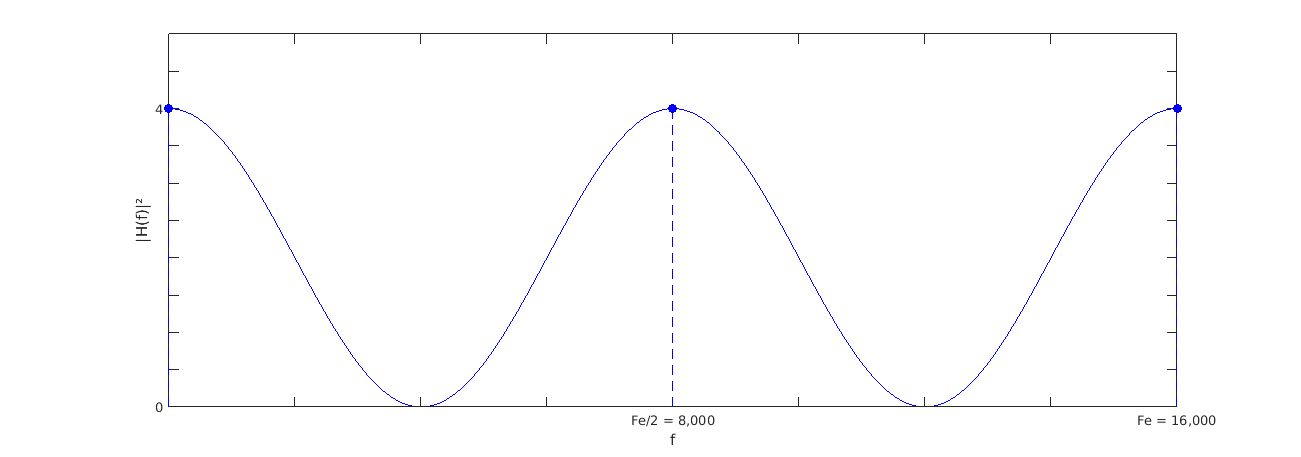
\includegraphics[width=1\textwidth]{img/modulePeigneDpairFull}
			\label{fig:modulePeigneDpair}
			\caption{Module de la fonction de transfert du filtre peigne avec D pair}
		\end{center}
\end{figure}

\begin{figure}[!ht]
		\begin{center}
			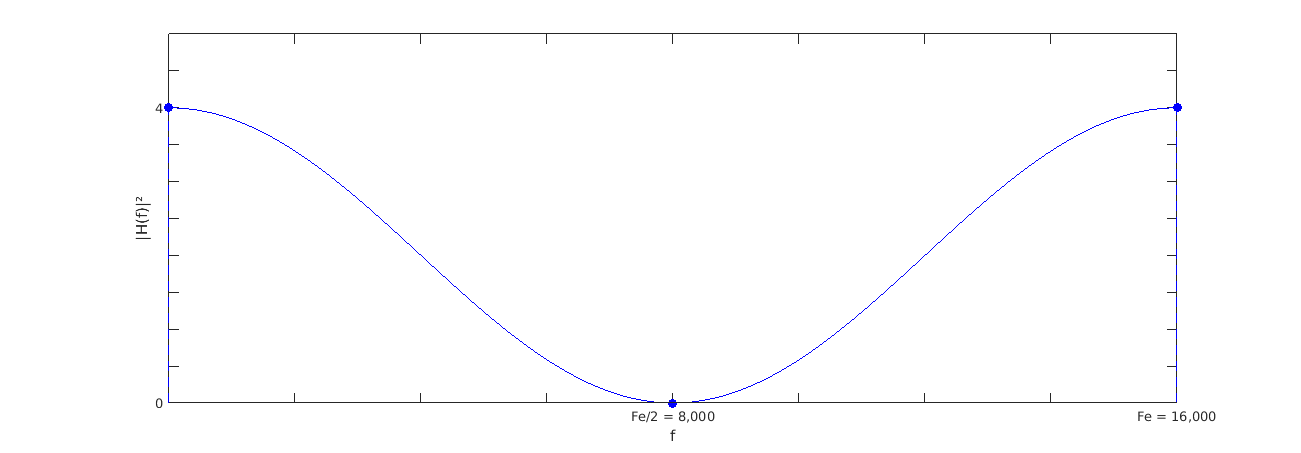
\includegraphics[width=1\textwidth]{img/modulePeigneDimpairFull}
			\label{fig:modulePeigneDimpair}
			\caption{Module de la fonction de transfert du filtre peigne avec D impair}
		\end{center}
\end{figure}

\clearpage

\subsection{Partie pratique}

- Etudier la fonction de transfert du filtre (impulsion en entrée). Etudier le module de la fonction de transfert. On prendra D=20

- Tester le filtre sur le signal audio avec différentes valeurs de D (de 20 à 5000). Quels sont les effets sonores observés ?

Pour $D = 5000$ le son est "dupliqué" avec un délai. On entend le son deux fois à quelques dixièmes de secondes d'intervalle. Lorsqu'on diminue les valeurs de D, le son reste dupliqué et joué en double avec un délai, mais ce-dernier est plus court. Pour $D = 20$, aucune différence n'est perçue à l'oreille nue.

\section{Filtre passe Tout}

\subsection{Partie théorique}

Soit le filtre passe-tout : $y(k) = −gx(k) + x(k − D) + gy(k − D)$

Donner la fonction de transfert en Z correspondant.

\begin{align*}
  &y(k) - gy(k - D) = -gk(k) + x(k - D)\\
  \iff &Y(Z) - gZ^{-D}Y(Z) = -gX(Z) + Z^{-D}X(Z)\\
  \iff &(1 - gZ^{-D})Y(Z) = (-g + Z^{-D})X(Z)\\
  \iff &Y(Z) = \frac{-g + Z^{-D}}{1 - gZ^{-D}}X(Z)\\
\end{align*}
Or, $Y(Z) = X(Z).H(Z)$ donc $H(Z) = \frac{-g + Z^{-D}}{1 - gZ^{-D}}$.\\

%passer par la forme somme des anx(k) - somme des bny(k)
%$H(Z) = -g + Z^{-D} + gZ

%- Dans quelles conditions ce filtre est-il stable ?

%\begin{align*}
%  &Filtre stable\\
%  \iff &somme |h(k)| < infini\\
%\end{align*}

%TODO

\subsection{Partie pratique}

- Etudier la fonction de transfert du filtre (impulsion en entrée). On prendra D=20 et g=0.5.\\
- Tester le filtre sur le signal audio avec différentes valeurs de D (de 20 à 5000). Quels sont les effets sonores observés ?

Pour $D = 5000$, on obtient un effet "echo" : le son se répète plusieurs fois avec un court délai (de l'ordre de quelques dixièmes de secondes) et de moins en moins fort. Lorsqu'on fait diminuer la valeur de D on obtient toujours un "echo" mais avec un délai plus court entre chaque itération du son entrant. Pour $D = 20$ il n'y a plus d'echo mais on remarque que le son en sortie sature bien moins que l'original : le bruit est beaucoup aténué.

\section{Réverbération}

Partie pratique
- La réverbération est obtenue grâce à la série de filtres suivante :
-Tester ce filtre sur le signal audio.
